%%%%%%%%%%%%%%%%%%%%%%%%%%%%%%%%%%%%%%%%%
% Simple Sectioned Essay Template
% LaTeX Template
%
% This template has been downloaded from:
% http://www.latextemplates.com
%
% Note:
% The \lipsum[#] commands throughout this template generate dummy text
% to fill the template out. These commands should all be removed when 
% writing essay content.
%
%%%%%%%%%%%%%%%%%%%%%%%%%%%%%%%%%%%%%%%%%

%----------------------------------------------------------------------------------------
%	PACKAGES AND OTHER DOCUMENT CONFIGURATIONS
%----------------------------------------------------------------------------------------

\documentclass[12pt]{article} % Default font size is 12pt, it can be changed here
\usepackage{hyperref}
\usepackage{multicol}
\usepackage{geometry} % Required to change the page size to A4
\geometry{a4paper} % Set the page size to be A4 as opposed to the default US Letter
\usepackage{graphicx} % Required for including pictures
\usepackage{float} % Allows putting an [H] in \begin{figure} to specify the exact location of the figure
\usepackage{wrapfig} % Allows in-line images such as the example fish picture
\linespread{1.2} % Line spacing
%\setlength\parindent{0pt} % Uncomment to remove all indentation from paragraphs
\graphicspath{{Pictures/}} % Specifies the directory where pictures are stored

\begin{document}

%----------------------------------------------------------------------------------------
%	TITLE PAGE
%----------------------------------------------------------------------------------------

\begin{titlepage}

\newcommand{\HRule}{\rule{\linewidth}{0.5mm}} % Defines a new command for the horizontal lines, change thickness here

\center % Center everything on the page

\textsc{\LARGE University of Southampton}\\[1.5cm] % Name of your university/college
\textsc{\Large Msc Cyber Security}\\[0.5cm] % Major heading such as course name
\textsc{\large Foundation of Data Science}\\[0.5cm] % Minor heading such as course title

\HRule \\[0.4cm]
{ \huge \bfseries Statistics with R}\\[0.4cm] % Title of your document
\HRule \\[1.5cm]

\begin{minipage}{0.4\textwidth}
\begin{flushleft} \large
\emph{Author:}\\
Gerard \textsc{Tio Nogueras} % Your name
\end{flushleft}
\end{minipage}
~
\begin{minipage}{0.4\textwidth}
\begin{flushright} \large
\emph{Supervisors:} \\
Pr. Elena  \textsc{Simperl}\\ % Supervisor's Name
Dr. Chris \textsc{Phethean}\\
Dr. Ramine \textsc{Tinati}\\
Dr. Markus \textsc{Brede}
\end{flushright}
\end{minipage}\\[4cm]

{\large \today}\\[3cm] % Date, change the \today to a set date if you want to be precise

%\includegraphics{Logo}\\[1cm] % Include a department/university logo - this will require the graphicx package

\vfill % Fill the rest of the page with whitespace
\end{titlepage}
\newpage
\section{First step: Distributions}
Different bin sizes:\\
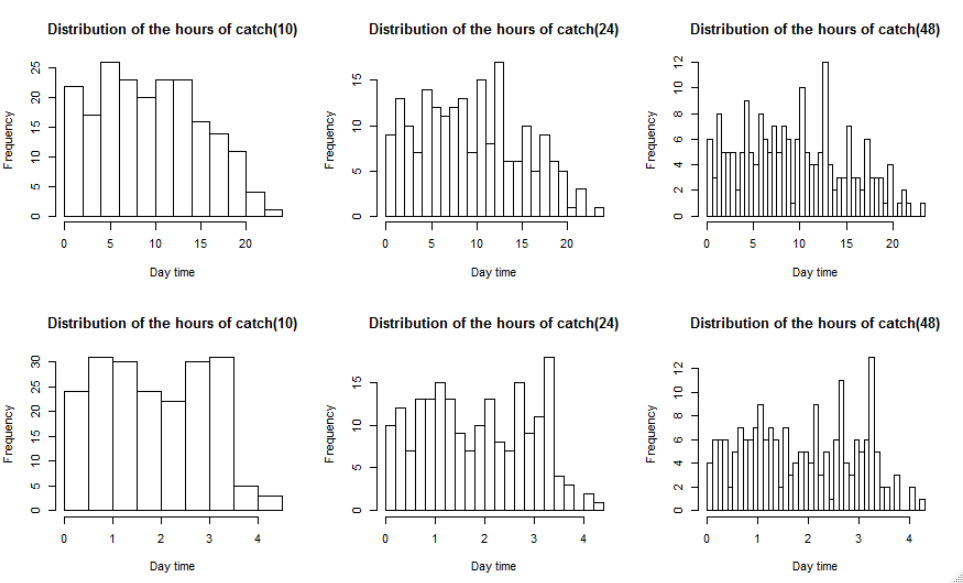
\includegraphics[scale=.55]{general_distributions}\\


\subsection{Typical Scores}
Freedman-Diaconis rule for bin sizes which gives us 2.8h for the times and 0.61kg for the weights.\\
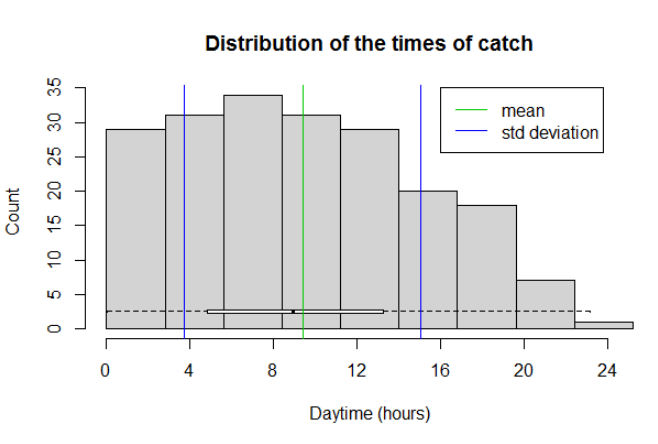
\includegraphics[scale=.45]{times_distribution}
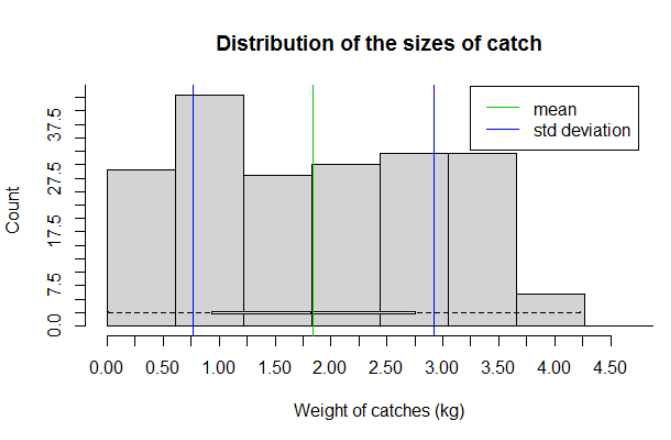
\includegraphics[scale=.45]{weights_distribution}
\newpage
\begin{multicols}{2}
\begin{tabular}{ll}
\textbf{Times}&\\
mean&9.388\\
median&8.950\\
mode&1.65\\
geometrical mean&6.786465\\
\end{tabular}
\\\\
\begin{tabular}{ll}
\textbf{Weights}&\\
mean&1.8431\\
median&1.8250\\
mode&3.22\\
geometrical mean&1.36948\\
\end{tabular}
\end{multicols}
We can see for both distributions that the means and the medians are almost equal this shows that each side of the median has the same total counts. The mode and geometrical mean are given as general information but I considered them irrelevant for this distributions because there are almost no repetitions in the dataset and the geometrical mean is mostly used to normalize different scales.\cite{mode}\cite{Geometric:mean}
\subsection{Range of Scores}
\begin{multicols}{2}
\begin{tabular}{ll}
\textbf{Times}&\\
minimum& 0.010\\
maximum& 23.160\\
variance& 31.99831\\
standard deviation& 5.656705\\
interquartile& range 8.335\\
skewness& 0.2477339\\
kurtosis& -0.8870124\\
\end{tabular}
\\\\
\begin{tabular}{ll}
\textbf{Weights}&\\
minimum& 0.0100\\
maximum& 4.2300\\
variance& 1.162248\\
standard deviation& 1.078076\\
interquartile& range 1.8\\
skewness& 0.08966\\
kurtosis& -1.169334\\
\end{tabular}
\end{multicols}
The IQR is smaller then the standard deviation range, this shows that the values between the first and the third quartile deviate less from the mean than the rest of the values. \\
For the time distribution, combining this with the fact that the mean and median are clearly on the left side of the center of 24h scope we expect similar counts between the standard deviation range and low counts for the right edge of the distribution.
For the weight distribution, combining the previous information with the mean and median values we expect a more uniformed distribution, which is the case with the exception of higher counts between 0.6kg and 1.25kg. This is balanced by the extreme right edge of the histogram which is really low.\cite{Standard_deviation}
\subsection{Kernel density estimation}
KDE allows for a smoother estimate of the distribution then the histogram. Normally this is used to extrapolate the PDF for a larger population.\cite{Kernel_density_estimation}\\\cite{Probability_density_function}\\
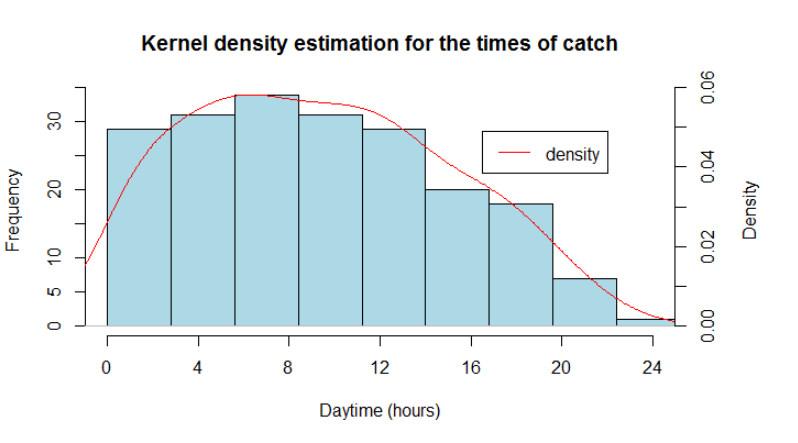
\includegraphics[scale=.4]{times_density}
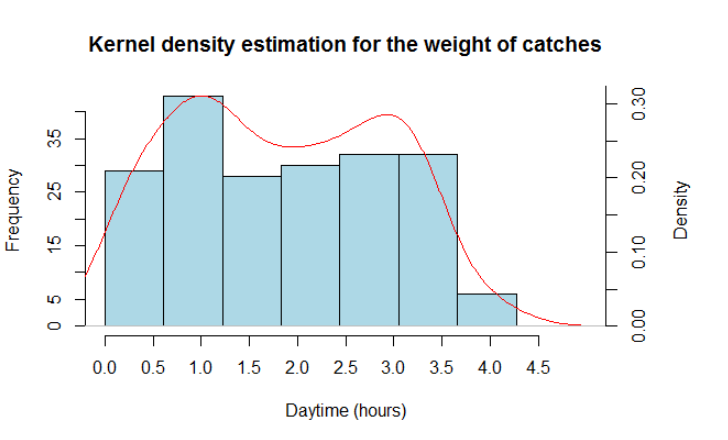
\includegraphics[scale=.4]{weights_density}
\subsection{Mean values with 95\% confidence intervals for both distributions}
The formula that will give us the confidence interval for population mean = $\bar{x}\pm z*s/\sqrt{n}$ with z being the z value for 95\% confidence interval, s the standard deviation of the sample, n the sample size and $\bar{x}$ the sample mean.
The confidence interval of the mean for the "times" is $[8.604371,10.17233]$ and for the weights it is $[1.693636,1.992464]$
\cite{Confidence_interval}\cite{Confidence_intervals_for_means}
\section{Second step: Correlation}
There isn't any apparent correlation, even when smooth scattering the distribution. After this approach we end up with a static snow distribution(no correlation).\\
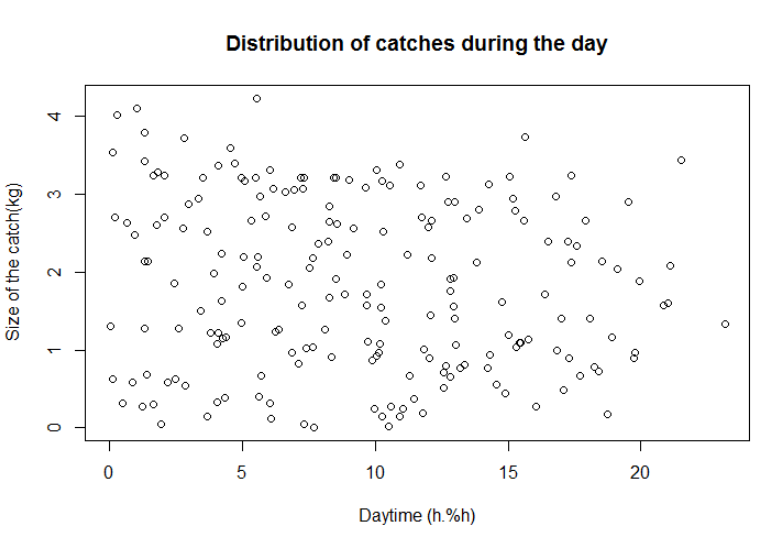
\includegraphics[scale=.4]{raw_correlation}
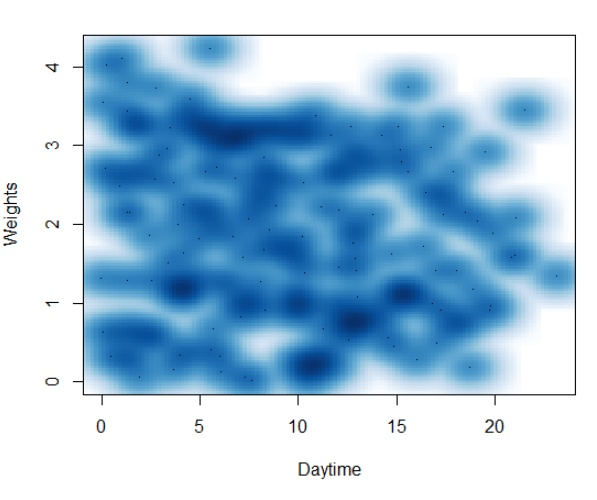
\includegraphics[scale=.4]{smoothscatter_correlation}
By regrouping the data by data frames of hours we can start retrieving interesting information. The median values before 10am are generally higher then the median of weights compared to the values after 10am which tend to have medians under weights median. In conclusion, the fishermen should go fish in the morning before 10am if they wish to obtain big catches.\\
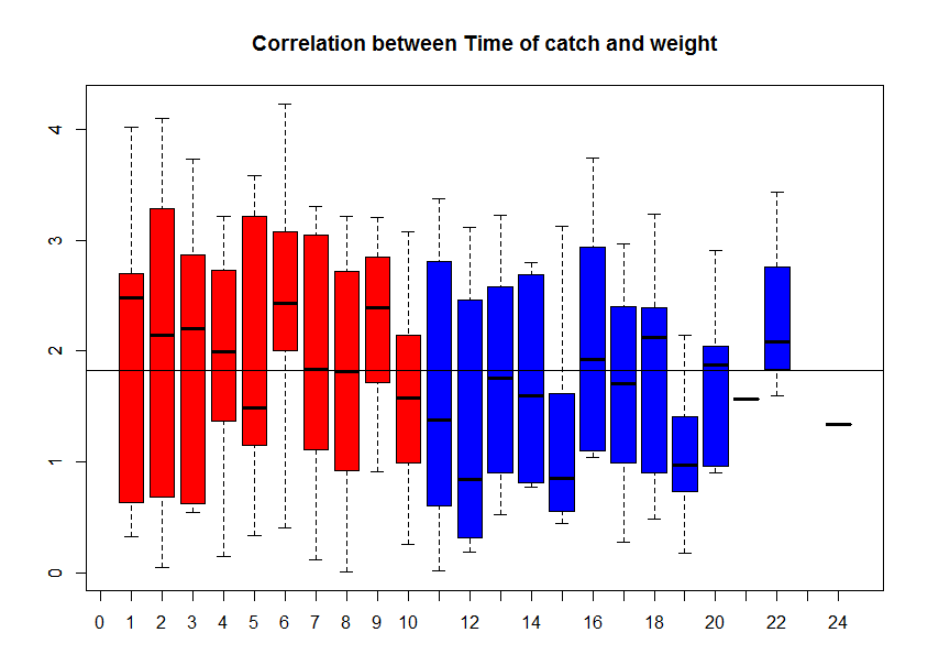
\includegraphics[scale=.6]{correlation}
The intervals with the lowest average rate of catching is $d$ and with the highest average is $d$.

\newpage
\begin{thebibliography}{99}
\bibitem[Geometric mean, 2016]{Geometric:mean} Geometric mean (2016) in Wikipedia. Available at: \url{https://en.wikipedia.org/wiki/Geometric_mean} (Accessed: 10 December 2016).

\bibitem[Mathsteacher, 2000]{mode}Mathsteacher (2000) Mean, median and mode. Available at: \url{http://www.mathsteacher.com.au/year8/ch17_stat/02_mean/mean.htm} (Accessed: 10 December 2016).

\bibitem [Standard deviation, 2016]{Standard_deviation}Standard deviation (2016) in Wikipedia. Available at: \url{https://en.wikipedia.org/wiki/Standard_deviation} (Accessed: 10 December 2016).

\bibitem[Kernel density estimation, 2016]{Kernel_density_estimation}Kernel density estimation (2016) in Wikipedia. Available at: \url{https://en.wikipedia.org/wiki/Kernel_density_estimation} (Accessed: 10 December 2016).

\bibitem [Probability density function, 2016]{Probability_density_function}Probability density function (2016) in Wikipedia. Available at: \url{https://en.wikipedia.org/wiki/Probability_density_function} (Accessed: 10 December 2016).

\bibitem[M. Lane, no date]{Confidence_interval} M. Lane, D. (no date) Confidence interval for the mean. Available at: \url{http://onlinestatbook.com/2/estimation/mean.html} (Accessed: 10 December 2016).

\bibitem[Confidence intervals for means, 2016]{Confidence_intervals_for_means}7.5 - confidence intervals for means (2016) Available at: \url{https://onlinecourses.science.psu.edu/stat200/node/49} (Accessed: 10 December 2016).

\end{thebibliography}

\end{document}